%%%%%%%%%%%%%%%%%%%%%%%%%%%%%%%%%%%%%%%%%
% University/School Laboratory Report
% LaTeX Template
% Version 2.0 (4/12/12)
%
% This template has been downloaded from:
% http://www.latextemplates.com
%
% License:
% CC BY-NC-SA 3.0 (http://creativecommons.org/licenses/by-nc-sa/3.0/)
%
% Original header:
%
% This is a LaTeX version of the sample laboratory report
% from Virginia Tech's copyrighted 08-09 CHEM 1045/1046 lab manual.
% Reproduction of this one appendix section for academic purposes
% should fall under fair use.
%
%%%%%%%%%%%%%%%%%%%%%%%%%%%%%%%%%%%%%%%%%

\documentclass{article}
\usepackage{graphicx}
\usepackage{float}
\usepackage{mathtools}

\title{ELEC 302-81\\ Lab 3\\ Non-Ideal Transformer Properties} % Title
% \author{John \textsc{Smith}} % Author name
\date{\today} % Specify a date for the report

\begin{document}

\maketitle

\begin{center}
  \begin{tabular}{lr}
    Date Performed: & February 4, 2013 \\
    Partners: & Rawley Dent \\
              & Charles Pittman \\
    Instructor: & Dr. Weatherford
  \end{tabular}
\end{center}

\pagebreak

%\setlength\parindent{0pt} % Removes all indentation from paragraphs

\section{Purpose of Experiment}
In this experiment, the basic characteristics of transformers were studied.
Various transformer circuits with different unknown turns ratios were
constructed in order to study the different voltage ratios at each particular
turns ratio. Other transformer circuits were constructed to observe the
similarity between the current ratio and turns ratio, and to observe the
saturation curve of a magnetic circuit.

\section{Procedure}
\subsection{EMS Workstation Set-up}

At the Lab-Volt EMS workstation, a Fluke multi-meter was used to measure the DC
resistance of each transformer winding. These values are recorded in
Table~\ref{tab:wind_res}.  The DAI 24V supply was turned on, and the DAI USB
connector was connected between the EMS workstation and the {PC}. On the LVDAM
EMS application software, the metering windows for E$_1$, E$_2$, E$_3$, I$_1$,
and I$_2$ were opened. The metering windows were set to continuous refresh.

\subsection{Transformer Performance}

\label{part1} With the main power switch to OFF and the voltage control knob
fully counterclockwise (CCW), the voltmeter selector switch was set to position
4--N. The circuit shown in Figure~\ref{fig:circuit_01}  was then constructed.
The main power switch was turned to ON and the voltage supply voltage was set
to 120V. The primary voltage was recorded from E$_1$ and the secondary voltage
was recorded from E$_2$.  The values for E$_1$ and E$_2$ were then measured and
recorded for each winding number listed in Table~\ref{tab:volt_rat}. The main
power switch was set to OFF and the voltage control knob was set fully CCW
before rewiring the circuit for each winding number. The respective turns ratio
for each set of winding number, primary, and secondary voltages was calculated
and also listed in Table~\ref{tab:volt_rat}. After completing the requisite
measurements, the main power switch was set OFF and the voltage control to
fully CCW.

\subsection{Open Circuit Test}

\label{part2} The circuit shown in Figure~\ref{fig:circuit_02} was then
constructed. The main power switch was set ON and the voltage control knob was
slowly adjusted to read 0.4A from I$_2$. It was noted that the ammeter I$_2$
shorted the windings 5--6.  Hence, extreme care was given to not exceed the
secondary winding current rating of 0.5A. The values for primary voltage E$_1$,
primary current I$_1$, and secondary current I$_2$ were then measured and
recorded, as shown in Table~\ref{tab:short_circ}.  The main power switch was set
OFF and the voltage control knob fully CCW.

\subsection{Short Circuit Test}

\label{part3} The circuit shown in Figure~\ref{fig:circuit_03} was then
constructed. The voltage supply connection was set from 4--N to 4--5. Since the
exciting current was small the 300$\Omega$ resistor was included and thus the
voltage E$_3$ across the resistor was used to show the current variation. On
the PC, the Data Table application was opened and set to record settings from
the Options tab. E$_1$, E$_2$, and E$_3$ appeared as the columns in the data
table. The main power switch was set ON and the supply voltage was then
increased in 10V increments from 0--180 volts. At each increment, the Record
Data tab was clicked to instantly enter the voltage measurements in the data
table. After reaching 180V, the main power switch was set to OFF and the
voltage supply control knob was fully {CCW}. On the {PC}, the Graph application
was opened.  E$_3$ (the exciting current) was set as the x-axis, and E$_1$ (the
applied voltage) as the y-axis. The Line Graph tab was clicked to display the
saturation curve of the transformer core.

\section{Results}
\subsection{Transformer Performance}
\begin{table}[H]
  \centering
  \begin{tabular}{*{2}{c}}
    \textbf{Winding} & \textbf{Resistance} \\
    \textbf{\#} & $\Omega$ \\
    \hline
    1--2 &  7.9 \\
    5--6 &  7.9 \\
  \end{tabular}
  \caption{Winding Resistances}
  \label{tab:wind_res}
\end{table}

\begin{table}[H]
  \centering
  \begin{tabular}{*{7}{c}}
    & \multicolumn{2}{c}{\textbf{Primary}} & \textbf{Input}
    & \multicolumn{2}{c}{\textbf{Secondary}} & \textbf{Output} \\
    \textbf{Load} & \textbf{Voltage} & \textbf{Current} & \textbf{Power}
    & \textbf{Voltage} & \textbf{Current} & \textbf{Power} \\
    Z$_\text{L}$ $\Omega$ & E$_1$ V & I$_1$ A & P$_1$ W
    & E$_2$ V & I$_2$ A &
    P$_2$ W \\
    \hline
    $\infty$   & 119.9 & 0.027 & 2.453 & 119.0 & 0.003 & 0 \\
    300        & 119.3 & 0.388 & 46.01 & 112.4 & 0.368 & 41.35 \\
    300 + j300 & 119.5 & 0.270 & 23.63 & 112.4 & 0.244 & 20.20 \\
    300 - j300 & 119.5 & 0.281 & 27.30 & 120.0 & 0.276 & 23.52 \\
  \end{tabular}
  \caption{Primary and secondary voltages and currents}
  \label{tab:volt_rat}
\end{table}

\subsection{Open Circuit Test}
\begin{table}[H]
  \centering
  \begin{tabular}{*{3}{c}}
    \multicolumn{2}{c}{\textbf{Primary}} & \textbf{Input} \\
    \textbf{Voltage} & \textbf{Current} & \textbf{Power} \\
    E$_1$ V & I$_1$ A & P$_2$ W \\
    \hline
    119.7 & 0.027 & 2.44 \\
  \end{tabular}
  \caption{Open Circuit}
  \label{tab:open_circ}
\end{table}

\subsection{Short Circuit Test}
\begin{table}[H]
  \centering
  \begin{tabular}{*{4}{c}}
    \multicolumn{2}{c}{\textbf{Primary}} & \textbf{Input} & \textbf{Secondary} \\
    \textbf{Voltage} & \textbf{Current} & \textbf{Power} & \textbf{Current} \\
    E$_1$ V & I$_1$ A & P$_1$ W & I$_2$ A \\
    \hline
    11.7 & 0.403 & 2.607 & 0.398 \\
  \end{tabular}
  \caption{Data for Fig~\ref{fig:circuit_03}}
  \label{tab:short_circ}
\end{table}

\section{Conclusions}

By measuring the resistance of each transformer winding and not getting any
extremely high resistance readings similar to an open circuit, it was
determined that the transformer windings had no faults and the integrity of the
windings were intact.

By measuring the voltage ratios for each particular transformer winding, the
turns ratio for that winding was calculated by taking the primary voltage over
the secondary voltage. This was one method to determine the turns ratio of an
unspecified transformer.

By measuring the current ratio for one set of transformer windings, another
method to determine the turns ratio was implemented. By referring to the text
\emph{Electric Machinery Fundamentals}, the current ratio of a transformer is
inversely proportional to the turns ratio. The relationship states:
$\frac{I_p}{I_s} = \frac{N_s}{N_p}$, where I$_\text{p}$ is the primary current,
I$_\text{s}$ the secondary current, N$_\text{p}$ the primary winding, and
N$_\text{s}$ the secondary winding.  The ratio of secondary current I$_2$ over
primary current I$_1$ was the same as the turns ratio calculated and recorded
in row 2 of Table~\ref{tab:volt_rat} pertaining to winding number 5--6.
Therefore, the additional method of determining a transformer turns ratio was
verified.

By analyzing the saturation curve, it was determined that the transformer core
did indeed become saturated.  From an applied voltage of 10V to approximately
110V, the saturation curve was linear and the transformer core was unsaturated
at this time. A small increase in the magneto-motive force (represented as
E$_3$) resulted in a very large increase in the flux produced (represented as
E$_1$).  Then the saturation curve started to level off after an applied
voltage of 110V (termed the \emph{knee} of the curve), and therefore the core
started to become saturated. In the saturated region, increases in
magneto-motive force produce smaller and smaller increases in flux.

\pagebreak
\section*{Circuits Tested}
\subsection*{Transformer Performance}
\begin{figure}[H]
  \centering
  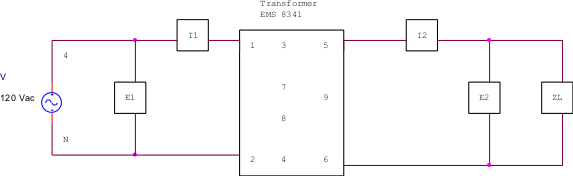
\includegraphics[width=.8\textwidth]{img/circuit_01}
  \caption{Single Phase Transformer Circuit for part one}
  \label{fig:circuit_01}
\end{figure}

\subsection*{Open Circuit Test}
\begin{figure}[H]
  \centering
  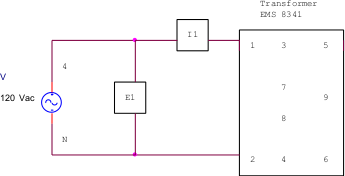
\includegraphics[width=.8\textwidth]{img/circuit_02}
  \caption{Single Phase Transformer Circuit for part two (open circuit test)}
  \label{fig:circuit_02}
\end{figure}

\subsection*{Short Circuit Test}
\begin{figure}[H]
  \centering
  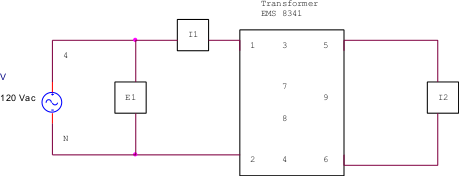
\includegraphics[width=.8\textwidth]{img/circuit_03}
  \caption{Single Phase Transformer Circuit for part two (short circuit test)}
  \label{fig:circuit_03}
\end{figure}

\end{document}
